\documentclass[a4]{article}
\usepackage{amssymb}
\usepackage{amsmath}
\usepackage{bm}
\usepackage{graphicx}

\DeclareMathOperator*{\argmax}{argmax}
\DeclareMathOperator*{\argmin}{argmin}

%opening
\title{Quick Refresher on HMM and LDS}
\author{Shoichiro Yamanishi}

\begin{document}

\maketitle

\begin{abstract}
This is a personal notes as my own memory aid on Hidden Markov Models and Linear Dynamical Systems.
Specifically the following topics.
\begin{itemize}
\item Baum-Welch EM algorithm 
\item Viterbi algorithm
\item Kalman Filter
\item Rauch-Tung-Striebel smoother and EM algorithm
\end{itemize}

Chapter 13 of PRML\cite{bishop2007} Chap 13 is an excellent source for HMM (Baum-Welch, Viterbi)
and Kalman Filter as in $p(\bm{z}_n| \bm{z}1, \cdots, \bm{z}_n)$, but not so good for
Kalman smoother (RTS smoother) as in $p(\bm{z}_n| \bm{z}_1, \cdots, \bm{z}_N)$.
Especially the derivation of  $p(\bm{z}_n, \bm{z}_{n+1}| \bm{z}_1, \cdots, \bm{z}_N)$, 
which is required for EM-algorithm, is a bit shaky between (13.103) and (13.104).
For deriving RTS smoother, I used an excellent course notes \cite{sarkka2011} from Professor S{\"a}rkk{\"a}
of Aalto Univ.
Also, Chap 24 of Barber \cite{Barber2011} contains comprehensive materials for LDS,
but it is a bit difficult to understand and I personally do not like the style of notations.
\end{abstract}

\section{Baum-Welch Algorithm}
\subsection{HMM Model formation}

\begin{figure}[!htb]
\centering
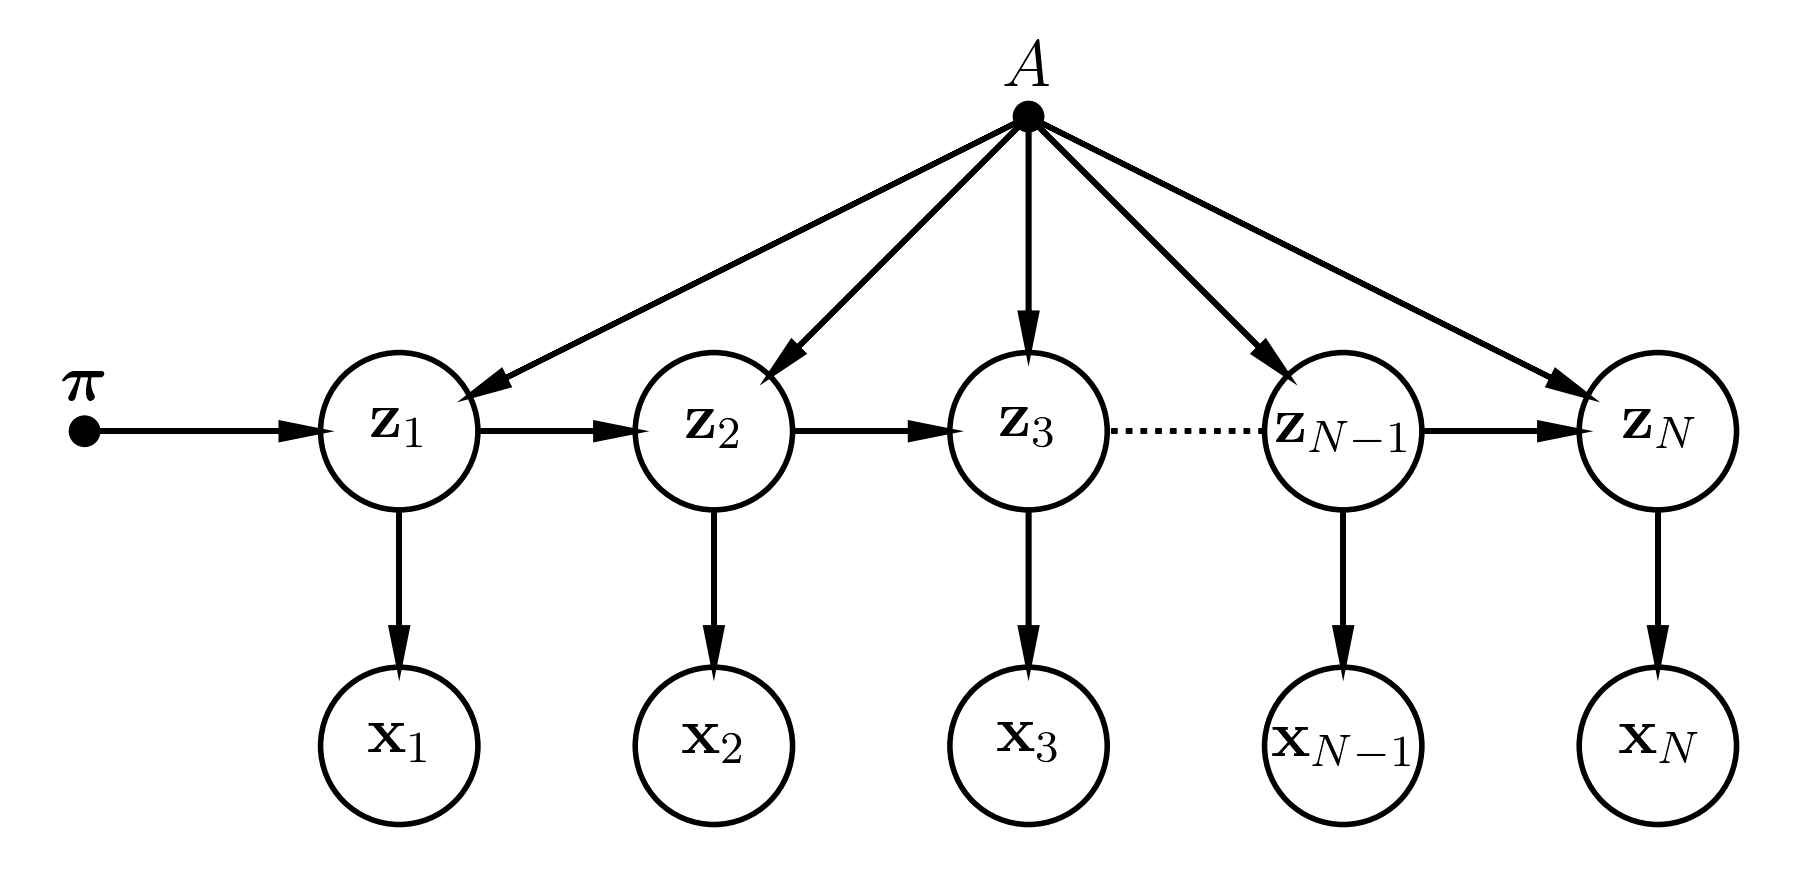
\includegraphics[width=8cm]{chain_discrete.png}
\caption{Parameter Reduction}
\label{fig:chain_discrete}
\end{figure}

Let $\bm{x}_i$ be the variables observed, and $\bm{z}_i$ be one-of-K latent variables.
And let the joint distribution be:
\begin{equation}
\begin{aligned}
p(\bm{x}_1, \bm{x}_2, \cdots, \bm{x}_N, \bm{z}_1, \bm{z}_2, \cdots, \bm{z}_N) = 
p(\bm{z}_1| \bm{\pi})\prod_{n=1}^N p(\bm{z}_n|\bm{z}_{n-1})\prod_{n=1}^N p(\bm{x}_n|\bm{z}_{n})
\label{eq:chain_model}
\end{aligned}
\end{equation}
as a hidden Markov model.
Please note that $(\bm{x}_1, \bm{x}_2, \cdots, \bm{x}_N)$ are not i.i.d.
We parameterize $p(\bm{z}_n|\bm{z}_{n-1})$ called \textit{transition probability} as $p(\bm{z}_n|\bm{z}_{n-1}, A)$,
where $A$ is a $K \times K$ matrix, and each row $A_i$ represent a multinomial distribution, i.e.,
$\sum_{j=1}^K A_{i,j} = 1$, and $A_{i,j} \ge 0$. This means $A_i$ represents the distribution of $\bm{z}_n$, 
if $[\bm{z}_{n-1}]_i =1$ ($i$ is chosen for $\bm{z}_{n-1}$.)
So, 
\begin{equation}
\begin{aligned}
p(\bm{z}_n|\bm{z}_{n-1}, A) = \prod_{j=1}^K\prod_{i=1}^K A_{i,j}^{[\bm{z}_{n-1}]_i[\bm{z}_{n}]_j}
\end{aligned}
\end{equation}
and for the initial distribution,
\begin{equation}
\begin{aligned}
p(\bm{z}_1|\bm{\pi}) = \prod_{j=1}^K {\pi}_j^{[\bm{z}_1]_j}
\end{aligned}
\end{equation}
We also parameterize $p(\bm{x}_n|\bm{z}_{n})$ called \textit{emission probability} as 
\begin{equation}
\begin{aligned}
p(\bm{x}_n|\bm{z}_{n}, \bm{\phi}) = \prod_{j=1}^K p(\bm{x}_n|\phi_{j})^{[\bm{z}_n]_j}
\end{aligned}
\end{equation}
This can be a Gaussian mixture.
Then we aggregate the parameters $A$ and $\bm{\phi}$ into $\bm{\theta}$
The parameterized joint distribution is:
\begin{equation}
\begin{aligned}
p(\bm{x}_1, \bm{x}_2, \cdots, \bm{x}_N, \bm{z}_1, \bm{z}_2, \cdots, \bm{z}_N|\bm{\theta}) = 
p(\bm{z}_1| \bm{\pi})\prod_{n=1}^N p(\bm{z}_n|\bm{z}_{n-1},A)\prod_{n=1}^N p(\bm{x}_n|\bm{z}_{n}, \bm{\phi})
\label{eq:chain_discrete}
\end{aligned}
\end{equation}

\subsection{Maximum Likelihood with EM-algorithm}
The maximum likelihodd estimate for the parameter $\bm{\theta}$ given the observations
$\bm{x}_1, \bm{x}_2, \cdots, \bm{x}_N$ is:
\begin{equation}
\begin{aligned}
\underset{\bm{\theta}}{\mathrm{argmax}} \left\{ p(\bm{x}_1, \bm{x}_2, \cdots, \bm{x}_N|\bm{\theta})  \right\} = 
\underset{\bm{\theta}}{\mathrm{argmax}} \left\{ \sum_{\bm{z}_1, \bm{z}_2, \cdots, \bm{z}_N}
p(\bm{x}_1, \bm{x}_2, \cdots, \bm{x}_N, \bm{z}_1, \bm{z}_2, \cdots, \bm{z}_N |\bm{\theta})  \right\}
\end{aligned}
\end{equation}
The summation over $\bm{z}_1, \bm{z}_2, \cdots, \bm{z}_N$ on RHS is intractable, and we need to use EM-framework.
For that we need to form the following function of $\bm{\theta}$ and $\bm{\theta}^*$ derived from ELBO.

\begin{equation}
\begin{aligned}
Q(\bm{\theta}_{old}, \bm{\theta}) &= \mathbb{E}_{(\bm{z}_1, \cdots, \bm{z}_N) \sim 
p(\bm{z}_1, \cdots, \bm{z}_N |\bm{x}_1, \cdots, \bm{x}_N, \bm{\theta}_{old})}\left[
\ln p(\bm{z}_1, \cdots, \bm{z}_N ,\bm{x}_1, \cdots, \bm{x}_N, \bm{\theta})
\right]\\
&=
\mathbb{E}\left[
\sum_{k=1}^K[\bm{z}_1]_k \ln \pi_k + 
\sum_{n=2}^N\sum_{j=1}^K\sum_{i=1}^K [\bm{z}_{n-1}]_i[\bm{z}_{n}]_j \ln A_{i,j} + 
\sum_{n=1}^N\sum_{i=1}^K [\bm{z}_{n-1}]_i \ln p(\bm{x}_n|\phi_k) \right]\\
&=
\sum_{k=1}^K
\mathbb{E}\left[[\bm{z}_1]_k\right] \ln \pi_k + 
\sum_{n=2}^N\sum_{j=1}^K\sum_{i=1}^K \mathbb{E}\left[
 [\bm{z}_{n-1}]_i[\bm{z}_{n}]_j \right]
 \ln A_{i,j} + 
\sum_{n=1}^N\sum_{i=1}^K \mathbb{E}\left[ [\bm{z}_{n}]_i \right] \ln p(\bm{x}_n|\phi_k)
\end{aligned}
\end{equation}
We introduce two types of marginal distributions,
\begin{equation}
\begin{aligned}
\bm{\gamma}(\bm{z}_i) &= p(\bm{z}_i|\bm{x}_1, \cdots, \bm{x}_N, \bm{\theta}_{old})\text{,} \in \mathcal{R}^K\\
\bm{\xi}(\bm{z}_i, \bm{z}_{i+1}) &=
 p(\bm{z}_i, \bm{z}_{i+1}|\bm{x}_1, \cdots, \bm{x}_N, \bm{\theta}_{old}) \in \mathcal{R}^{K\times K}
\end{aligned}
\end{equation}
as in (13.13) and (13.14) of PRML \cite{bishop2007}.
Then we can express the expectations above as follows.
\begin{equation}
\begin{aligned}
\mathbb{E}\left[[\bm{z}_i]_k\right] &= \sum_{k=1}^K[\bm{\gamma}(\bm{z}_i)]_k[\bm{z}_i]_k\\
\mathbb{E}\left[[\bm{z}_i]_k [\bm{z}_{i+1}]_m\right] &= \sum_{k=1}^K \sum_{m=1}^K
[\bm{\xi}(\bm{z}_i, \bm{z}_{i+1})]_{km}[\bm{z}_i]_k[\bm{z}_{i+1}]_m
\end{aligned}
\end{equation}

Please note $p(\bm{z}_1, \cdots, \bm{z}_N |\bm{x}_1, \cdots, \bm{x}_N, \bm{\theta}_{old})$ is not cleanly factorized,
i.e. Marginalization is required for 
$\bm{\gamma}(\bm{z}_i)$ and $\bm{\xi}(\bm{z}_i, \bm{z}_{i+1})$.
This is where the sum-product belief propagaion along the chain comes to the rescue.

First we factorize $\bm{\gamma}(\bm{z}_n)$ conditioned on $\bm{x}_1, \cdots, \bm{x}_N$.
using Baye's rule and the conditional independence.
\begin{equation}
\begin{aligned}
\bm{\gamma}(\bm{z}_n) &= p(\bm{z}_n|\bm{x}_1, \cdots, \bm{x}_N)\\
&= \frac{
    p(\bm{x}_1, \cdots, \bm{x}_N | \bm{z}_n) p(\bm{z}_n)
}
{
    p(\bm{x}_1, \cdots, \bm{x}_N)
}\\
&= \frac{
    p(\bm{x}_1, \cdots, \bm{x}_n | \bm{z}_n)
    p(\bm{x}_{n+1}, \cdots, \bm{x}_N | \bm{z}_n)p(\bm{z}_n)
}
{
    p(\bm{x}_1, \cdots, \bm{x}_N)
}\\
&= \frac{
    p(\bm{x}_1, \cdots, \bm{x}_n, \bm{z}_n)
    p(\bm{x}_{n+1}, \cdots, \bm{x}_N | \bm{z}_n)
}
{
    p(\bm{x}_1, \cdots, \bm{x}_N)
}\\
&= \frac{
    \bm{\alpha}(\bm{z}_n)
    \bm{\beta}(\bm{z}_n)
}
{
    p(\bm{x}_1, \cdots, \bm{x}_N)
}
\end{aligned}
\end{equation}
where 
$\bm{\alpha}(\bm{z}_n) = p(\bm{x}_1, \cdots, \bm{x}_n, \bm{z}_n)$
and 
$\bm{\beta}(\bm{z}_n) = p(\bm{x}_{n+1}, \cdots, \bm{x}_N | \bm{z}_n)$.

In the same way, we factorize $\bm{\xi}(\bm{z}_i, \bm{z}_{i+1})$ conditioned on $\bm{x}_1, \cdots, \bm{x}_N$.
\begin{equation}
\begin{aligned}
\bm{\xi}(\bm{z}_n, \bm{z}_{n+1}) &= p(\bm{z}_n, \bm{z}_{n+1}|\bm{x}_1, \cdots, \bm{x}_N)\\
&= \frac{
    p(\bm{x}_1, \cdots, \bm{x}_N , \bm{z}_n, \bm{z}_{n+1})
}
{
    p(\bm{x}_1, \cdots, \bm{x}_N)
}\\
&= \frac{
    p(\bm{x}_1, \cdots, \bm{x}_N | \bm{z}_{n}, \bm{z}_{n+1})p(\bm{z}_n, \bm{z}_{n+1})
}
{
    p(\bm{x}_1, \cdots, \bm{x}_N)
}\\
&= \frac{
    p(\bm{x}_1,     \cdots, \bm{x}_n | \bm{z}_{n}, \bm{z}_{n+1})
    p(\bm{x}_{n+1}                   | \bm{z}_{n}, \bm{z}_{n+1})
    p(\bm{x}_{n+2}, \cdots, \bm{x}_N | \bm{z}_{n}, \bm{z}_{n+1})p(\bm{z}_{n+1} | \bm{z}_{n}) p(\bm{z}_{n})
}
{
    p(\bm{x}_1, \cdots, \bm{x}_N)
}\\
&= \frac{
    p(\bm{x}_1,     \cdots, \bm{x}_n | \bm{z}_{n} )
    p(\bm{x}_{n+1}                   | \bm{z}_{n+1})
    p(\bm{x}_{n+2}, \cdots, \bm{x}_N | \bm{z}_{n+1})p(\bm{z}_{n+1} | \bm{z}_{n}) p(\bm{z}_{n})
}
{
    p(\bm{x}_1, \cdots, \bm{x}_N)
}\\
&= \frac{
    p(\bm{x}_1,     \cdots, \bm{x}_n | \bm{z}_{n} ) p(\bm{z}_{n})
    p(\bm{x}_{n+1}                   | \bm{z}_{n+1})p(\bm{z}_{n+1} | \bm{z}_{n})
    p(\bm{x}_{n+2}, \cdots, \bm{x}_N | \bm{z}_{n+1})
}
{
    p(\bm{x}_1, \cdots, \bm{x}_N)
}\\
&= \frac{
    \bm{\alpha}(\bm{z}_n)
    p(\bm{x}_{n+1} | \bm{z}_{n+1})p(\bm{z}_{n+1} | \bm{z}_{n})
    \bm{\beta}(\bm{z}_{n+1})
}
{
    p(\bm{x}_1, \cdots, \bm{x}_N)
}\\
\end{aligned}
\end{equation}

\subsection{Belief Propagation (Sum-Product Algorithm over a Chain}
Next we define  $\bm{\alpha}(\bm{z}_n)$ in the forward propagation, and $\bm{\beta}(\bm{z}_{n})$ in the
backward propagation as follows.

\begin{equation}
\begin{aligned}
\bm{\alpha}(\bm{z}_1) &= p(\bm{x}_1, \bm{z}_1) = p(\bm{x}_1|\bm{z}_1)p(\bm{z}_1)\\
\bm{\alpha}(\bm{z}_n) &= p(\bm{x}_1, \cdots, \bm{x}_n , \bm{z}_n)\\
                      &= p(\bm{x}_1, \cdots, \bm{x}_n | \bm{z}_n)p(\bm{z}_n)\\
                      &= p(\bm{x}_{n}|\bm{z}_n) p(\bm{x}_1, \cdots, \bm{x}_{n-1}| \bm{z}_n)p(\bm{z}_n)\\
                      &= p(\bm{x}_{n}|\bm{z}_n) p(\bm{x}_1, \cdots, \bm{x}_{n-1}, \bm{z}_n)\\
                      &= p(\bm{x}_{n}|\bm{z}_n) 
                         \sum_{k=1}^K p(\bm{x}_1, \cdots, \bm{x}_{n-1}, [\bm{z}_{n-1}]_k, \bm{z}_n )\\
                      &= p( \bm{x}_{n} | \bm{z}_n ) 
                         \sum_{k=1}^K p( \bm{x}_1, \cdots, \bm{x}_{n-1}, \bm{z}_n \:|\: [\bm{z}_{n-1}]_k )
                         p( [\bm{z}_{n-1}]_k )\\
                      &= p( \bm{x}_{n} | \bm{z}_n ) 
                         \sum_{k=1}^K p( \bm{x}_1, \cdots, \bm{x}_{n-1} \:|\: [\bm{z}_{n-1}]_k )
                                      p( \bm{z}_n \:|\: [\bm{z}_{n-1}]_k )
                         p( [\bm{z}_{n-1}]_k )\\
                      &= p( \bm{x}_{n} | \bm{z}_n ) 
                         \sum_{k=1}^K p( \bm{x}_1, \cdots, \bm{x}_{n-1}\: |\: [\bm{z}_{n-1}]_k )p( [\bm{z}_{n-1}]_k )
                                      p( \bm{z}_n \:|\: [\bm{z}_{n-1}]_k )\\
                      &= p( \bm{x}_{n} | \bm{z}_n ) 
                         \sum_{k=1}^K [\bm{\alpha}(\bm{z}_{n-1})]_k p( \bm{z}_n \:|\ [\bm{z}_{n-1}]_k )\label{eq:definition_alpha}\\
\end{aligned}
\end{equation}
This is a forward propagation summing over $\bm{z}_{n-1}$.
Please note $\bm{\alpha}(\bm{z}_n)$ is not a normalized probability distribution.
In the same way, 

\begin{equation}
\begin{aligned}
\bm{\beta}(\bm{z}_N) &= \bm{1}\\
\bm{\beta}(\bm{z}_n) &= p(\bm{x}_{n+1}, \cdots, \bm{x}_N | \bm{z}_n)\\
                     &= \frac{p(\bm{x}_{n+1}, \cdots, \bm{x}_N , \bm{z}_n)}{p(\bm{z}_n)}\\
                     &= \frac{
                          \sum_{k=1}^K p(\bm{x}_{n+1}, \cdots, \bm{x}_N , \bm{z}_n, [\bm{z}_{n+1}]_k)
                        }{p(\bm{z}_n)}\\
                     &= \frac{
                          \sum_{k=1}^K  p(\bm{x}_{n+1}, \cdots, \bm{x}_N , \bm{z}_n \:|\: [\bm{z}_{n+1}]_k)
                          p( [\bm{z}_{n+1}]_k )
                        }{p(\bm{z}_n)}\\
                     &= \frac{
                          \sum_{k=1}^K
                              p( \bm{x}_{n+1}, \cdots, \bm{x}_N \:|\: [\bm{z}_{n+1}]_k )
                              p( \bm{z}_n \:|\: [\bm{z}_{n+1}]_k )
                              p( [\bm{z}_{n+1}]_k )
                        }{p(\bm{z}_n)}\\
                     &= \frac{
                          \sum_{k=1}^K
                              p( \bm{x}_{n+1}, \cdots, \bm{x}_N \:|\: [\bm{z}_{n+1}]_k )
                              p( \bm{z}_n, [\bm{z}_{n+1}]_k )
                        }{p(\bm{z}_n)}\\
                     &= \frac{
                          \sum_{k=1}^K
                              p( \bm{x}_{n+1}, \cdots, \bm{x}_N \:|\: [\bm{z}_{n+1}]_k )
                              p( [\bm{z}_{n+1}]_k |\bm{z}_n )  p(\bm{z}_n )
                        }{p(\bm{z}_n)}\\
                     &= \frac{
                            p(\bm{z}_n )\sum_{k=1}^K
                              p( \bm{x}_{n+1}, \cdots, \bm{x}_N \:|\: [\bm{z}_{n+1}]_k )
                              p( [\bm{z}_{n+1}]_k |\bm{z}_n )
                        }{p(\bm{z}_n)}\\
                     &=
                        \sum_{k=1}^K
                              p( \bm{x}_{n+1}, \cdots, \bm{x}_N \:|\: [\bm{z}_{n+1}]_k )
                              p( [\bm{z}_{n+1}]_k |\bm{z}_n )\\
                     &=
                        \sum_{k=1}^K
                              p( \bm{x}_{n+1} \:|\: [\bm{z}_{n+1}]_k )
                              p( \bm{x}_{n+2}, \cdots, \bm{x}_N \:|\: [\bm{z}_{n+1}]_k )
                              p( [\bm{z}_{n+1}]_k |\bm{z}_n )\\
                     &=
                        \sum_{k=1}^K
                              \bm{\beta}(\bm{z}_{n+1})
                              p( \bm{x}_{n+1} \:|\: [\bm{z}_{n+1}]_k )
                              p( [\bm{z}_{n+1}]_k |\bm{z}_n )\label{eq:definition_beta},\\
\end{aligned}
\end{equation}
This is a backward propagation summing over $\bm{z}_{n+1}$.
Please note that the derivation of $\beta(\bm{z}_n)$ in PRML \cite{bishop2007}
in pp 621 is wrong between the 2nd and 3rd lines.

After finding $\alpha(\bm{z}_n)$ and $\beta(\bm{z}_n)$, we can calculate 
$\bm{\gamma}(\bm{z}_n)$ and $\bm{\xi}(\bm{z}_n, \bm{z}_{n+1})$, and then
$\mathbb{E}\left[[\bm{z}_i]_k\right]$ and $\mathbb{E}\left[[\bm{z}_i]_k [\bm{z}_{i+1}]_m\right]$.
This corresponds to the E-step.

Then at the M-step, we can find $\bm{\theta}^*$ such that
$\bm{\theta}^* = \underset{\bm{\theta}}{\mathrm{argmax}} \left\{Q(\bm{\theta}_{old}, \bm{\theta})\right\}$.
Usually this is achieved by $\nabla_{\bm{\theta}}Q(\bm{\theta}_{old}, \bm{\theta}) = 0$.

\subsection{Scaling $\alpha$ and $\beta$}

As stated above, $\alpha(\bm{z}_n)$ and $\beta(\bm{z}_n)$ are not normalized and it can lead to numerical issues through the recursion.
To avoid those issues, we normalize  $\alpha(\bm{z}_n)$ and we increase the value of $\beta(\bm{z}_n)$ as follows.
\begin{equation}
\begin{aligned}
    \bm{\hat{\alpha}}(\bm{z}_n) = \frac{
        \bm{\alpha}(\bm{z}_n)
    }
    {
        p( \bm{x}_1, \cdots, \bm{x}_n )
    }
    = \frac{
        p( \bm{x}_1, \cdots, \bm{x}_n , \bm{z}_n )
    }
    {
        p( \bm{x}_1, \cdots, \bm{x}_n )
    }
    =
        p( \bm{z}_n | \bm{x}_1, \cdots, \bm{x}_n )
\end{aligned}
\end{equation}

\begin{equation}
\begin{aligned}
    \bm{\hat{\beta}}(\bm{z}_n) = \frac{
        \bm{\beta}(\bm{z}_n)
    }
    {
        p( \bm{x}_{n+1}, \cdots, \bm{x}_{N}| \bm{x}_1, \cdots, \bm{x}_n )
    }
    = \frac{
        p( \bm{x}_{n+1}, \cdots, \bm{x}_N  | \bm{z}_n )
    }
    {
        p( \bm{x}_{n+1}, \cdots, \bm{x}_{N}| \bm{x}_1, \cdots, \bm{x}_n )
    }
\end{aligned}
\end{equation}
Please note that $\bm{\hat{\alpha}}(\bm{z}_n)$ is a proper pribability density function, but
$\bm{\hat{\beta}}(\bm{z}_n)$ is not.
Next, we calculate $\bm{\hat{\alpha}}(\bm{z}_n)$ and $\bm{\hat{\beta}}(\bm{z}_n)$ recursively
with belief propagation. For that, use a a tool as a factor as follows.
\begin{equation}
\begin{aligned}
c_1 &= p(\bm{x}_1)\\
c_n &= p(\bm{x}_n | \bm{x}_1, \bm{x}_2, \cdots, \bm{x}_{n-1})
\end{aligned}
\end{equation}
It has the following characteristics.
\begin{equation}
\begin{aligned}
\prod_{i=1}^n c_i &= p(\bm{x}_1) p(\bm{x}_2|\bm{x}_1) p(\bm{x}_3|\bm{x}_1, \bm{x}_2)\cdots
p(\bm{x}_n|\bm{x}_1, \bm{x}_2, \cdots, \bm{x}_{n-1})\\
 &= 
p(\bm{x}_1)
\frac{ p(\bm{x}_2, \bm{x}_1) }{ p(\bm{x}_1) }
\frac{ p(\bm{x}_3, \bm{x}_2, \bm{x}_1) }{ p(\bm{x}_1,  \bm{x}_2) }
\cdots
\frac{ p(\bm{x}_n, \bm{x}_{n-1},\cdots, \bm{x}_1) }{p(\bm{x}_{n-1},\cdots, \bm{x}_1) }\\
&= p(\bm{x}_n, \bm{x}_{n-1},\cdots, \bm{x}_1)
\end{aligned}
\end{equation}
\begin{equation}
\begin{aligned}
\prod_{i={n+1}}^N c_i
&=
p(\bm{x}_{n+1}|\bm{x}_1, \cdots, \bm{x}_n)
p(\bm{x}_{n+2}|\bm{x}_1, \cdots, \bm{x}_{n+1})
\cdots
p(\bm{x}_{N}|\bm{x}_1, \cdots, \bm{x}_{N-1})\\
&=
\frac{p(\bm{x}_1, \cdots, \bm{x}_{n+1})}{p(\bm{x}_1, \cdots, \bm{x}_{n})}
\frac{p(\bm{x}_1, \cdots, \bm{x}_{n+2})}{p(\bm{x}_1, \cdots, \bm{x}_{n+1})}
\cdots
\frac{p(\bm{x}_1, \cdots, \bm{x}_{N})}{p(\bm{x}_1, \cdots, \bm{x}_{N-1})}\\
&= \frac{p(\bm{x}_1, \cdots, \bm{x}_{N})}{p(\bm{x}_1, \cdots, \bm{x}_{n})}\\
&= p(\bm{x}_{n+1}, \cdots, \bm{x}_{N} | \bm{x}_1, \cdots, \bm{x}_{n})
\end{aligned}
\end{equation}

Then analogous to the equatation \ref{eq:definition_alpha},
the recursive definision of $\bm{\hat{\alpha}}(\bm{z}_n)$ will be

\begin{equation}
\begin{aligned}
&
\:\:\:\:p( \bm{x}_{n} | \bm{z}_n ) 
\sum_{k=1}^K [\bm{\hat{\alpha}}(\bm{z}_{n-1})]_k p( \bm{z}_n \:|\ [\bm{z}_{n-1}]_k )\\
&=
p( \bm{x}_{n} | \bm{z}_n ) 
\sum_{k=1}^K \left[
\frac{\bm{\alpha}(\bm{z}_{n-1})}{p(\bm{x}_n, \cdots, \bm{x}_{n-1})}
\right]_k p( \bm{z}_n \:|\ [\bm{z}_{n-1}]_k )\\
&=
\frac{1}{p(\bm{x}_n, \cdots, \bm{x}_{n-1})}
p( \bm{x}_{n} | \bm{z}_n ) 
\sum_{k=1}^K \left[\bm{\alpha}(\bm{z}_{n-1})\right]_k p( \bm{z}_1 \:|\ [\bm{z}_{n-1}]_k )\\
&=
\frac{\bm{\alpha}(\bm{z}_{n})}{p(\bm{x}_1, \cdots, \bm{x}_{n-1})}\\
&=
\frac{ \bm{\hat{\alpha}}({\bm{z}_n})p(\bm{x}_1, \cdots, \bm{x}_{n}) }
     { p(\bm{x}_1, \cdots, \bm{x}_{n-1}) }\\
&=
\bm{\hat{\alpha}}({\bm{z}_n})p(\bm{x}_n | \bm{x}_1, \cdots, \bm{x}_{n-1})\\
&= c_n\bm{\hat{\alpha}}({\bm{z}_n})
\label{eq:definition_alpha_hat}\\
\end{aligned}
\end{equation}
Since $\bm{\hat{\alpha}}({\bm{z}_n})$ is a normalized distribution, we can calculate
$c_n$ as the partition function of RHS of \ref{eq:definition_alpha_hat} as follows.
\begin{equation}
\begin{aligned}
c_n = \sum_{k=1}^K [\bm{\hat{\alpha}}({\bm{z}_n})p(\bm{x}_n | \bm{x}_1, \cdots, \bm{x}_{n-1})]_k
\end{aligned}
\end{equation}

In the same way, for $\bm{\hat{\beta}}(\bm{z}_n)$, analogous to \ref{eq:definition_beta},
\begin{equation}
\begin{aligned}
&
\:\:\:\:
\sum_{k=1}^K [\bm{\hat{\beta}}(\bm{z}_{n+1})]_k 
p( \bm{x}_{n+1} | [\bm{z}_{n+1}]_k )[p([\bm{z}_{n+1} \:|\ [\bm{z}_{n})]_k\\
&=
\frac{
\sum_{k=1}^K [\bm{\beta}(\bm{z}_{n+1})]_k 
p( \bm{x}_{n+1} | [\bm{z}_{n+1}]_k )[p([\bm{z}_{n+1} \:|\ [\bm{z}_{n})]_k
}{p( \bm{x}_{n+2}, \cdots, \bm{x}_{N} | \bm{x}_{1}, \cdots, \bm{x}_{n+1} ) }\\
&=
\frac{
    \bm{\beta}(\bm{z}_{n})
}
{
    p( \bm{x}_{n+2}, \cdots, \bm{x}_{N} | \bm{x}_{1}, \cdots, \bm{x}_{n+1} )
}\\
&=
\frac{
    p( \bm{x}_{n+1}, \cdots, \bm{x}_{N} | \bm{x}_{1}, \cdots, \bm{x}_{n} )
}
{
    p( \bm{x}_{n+2}, \cdots, \bm{x}_{N} | \bm{x}_{1}, \cdots, \bm{x}_{n+1} )
}
\bm{\hat{\beta}}(\bm{z}_{n})\\
&=
\frac{
    \frac{
        p( \bm{x}_{1}, \cdots, \bm{x}_{N} )
    }
    {
        p( \bm{x}_{1}, \cdots, \bm{x}_{n} )
    }
}
{
    \frac{
        p( \bm{x}_{1}, \cdots, \bm{x}_{N} )
    }
    {
        p( \bm{x}_{1}, \cdots, \bm{x}_{n+1} )
    }
}
\bm{\hat{\beta}}(\bm{z}_{n})\\
&=
\frac{
    p( \bm{x}_{1}, \cdots, \bm{x}_{n+1} )
}
{
    p( \bm{x}_{1}, \cdots, \bm{x}_{n} )
}
\bm{\hat{\beta}}(\bm{z}_{n})\\
&=
p( \bm{x}_{n+1} | \bm{x}_{1}, \cdots, \bm{x}_{n} )\bm{\hat{\beta}}(\bm{z}_{n})\\
&=
c_{n+1}\bm{\hat{\beta}}(\bm{z}_{n})
\\
\end{aligned}
\end{equation}

Then 

\begin{equation}
\begin{aligned}
\bm{\gamma}(\bm{z}_n) &= p(\bm{z}_n|\bm{x}_1, \cdots, \bm{x}_N)
= \frac{
    \bm{\alpha}(\bm{z}_n)
    \bm{\beta}(\bm{z}_n)
}
{
    p(\bm{x}_1, \cdots, \bm{x}_N)
}\\
&= \frac{
    \bm{\hat{\alpha}}(\bm{z}_n)p(\bm{x}_1, \cdots, \bm{x}_n)
    \bm{\hat{\beta}}(\bm{z}_n)p(\bm{x}_{n+1}, \cdots, \bm{x}_N|\bm{x}_{1}, \cdots, \bm{x}_n)
}
{
    p(\bm{x}_1, \cdots, \bm{x}_N)
}\\
&= \frac{
    \bm{\hat{\alpha}}(\bm{z}_n)
    \bm{\hat{\beta}}(\bm{z}_n)p(\bm{x}_1, \cdots, \bm{x}_N)
}
{
    p(\bm{x}_1, \cdots, \bm{x}_N)
}\\
&= \bm{\hat{\alpha}}(\bm{z}_n)\bm{\hat{\beta}}(\bm{z}_n)
\end{aligned}
\end{equation}

and
\begin{equation}
\begin{aligned}
\bm{\xi}(\bm{z}_n, \bm{z}_{n+1})
&= p(\bm{z}_n, \bm{z}_{n+1}|\bm{x}_1, \cdots, \bm{x}_N)
= \frac{
    \bm{\alpha}(\bm{z}_n)
    p(\bm{x}_{n+1}|\bm{z}_{n+1})p(\bm{z}_{n+1}|\bm{z}_{n})
    \bm{\beta}(\bm{z}_{n+1})
}
{
    p(\bm{x}_1, \cdots, \bm{x}_N)
}\\
&= \frac{
    \bm{\hat{\alpha}}(\bm{z}_n)p(\bm{x}_1, \cdots, \bm{x}_n)
    p(\bm{x}_{n+1}|\bm{z}_{n+1})p(\bm{z}_{n+1}|\bm{z}_{n})
    \bm{\hat{\beta}}(\bm{z}_{n+1})
    p(\bm{x}_{n+2}, \cdots, \bm{x}_N|\bm{x}_{1}, \cdots, \bm{x}_{n+1})
}
{
    p(\bm{x}_1, \cdots, \bm{x}_N)
}\\
&= \frac{
    \bm{\hat{\alpha}}(\bm{z}_n)p(\bm{x}_1, \cdots, \bm{x}_n)
    p(\bm{x}_{n+1}|\bm{z}_{n+1})p(\bm{z}_{n+1}|\bm{z}_{n})
    \bm{\hat{\beta}}(\bm{z}_{n+1})
    p(\bm{x}_{1}, \cdots, \bm{x}_N)
}
{
    p(\bm{x}_1, \cdots, \bm{x}_N)    p(\bm{x}_1, \cdots, \bm{x}_{n+1})
}\\
&= \frac{
    \bm{\hat{\alpha}}(\bm{z}_n)p(\bm{x}_1, \cdots, \bm{x}_n)
    p(\bm{x}_{n+1}|\bm{z}_{n+1})p(\bm{z}_{n+1}|\bm{z}_{n})
    \bm{\hat{\beta}}(\bm{z}_{n+1})
}
{
    p(\bm{x}_1, \cdots, \bm{x}_{n+1})
}\\
&= \frac{
    \bm{\hat{\alpha}}(\bm{z}_n)
    p(\bm{x}_{n+1}|\bm{z}_{n+1})p(\bm{z}_{n+1}|\bm{z}_{n})
    \bm{\hat{\beta}}(\bm{z}_{n+1})
}
{
    p(\bm{x}_{n+1} | \bm{x}_1, \cdots, \bm{x}_{n})
}\\
&= \frac{
    \bm{\hat{\alpha}}(\bm{z}_n)
    p(\bm{x}_{n+1}|\bm{z}_{n+1})p(\bm{z}_{n+1}|\bm{z}_{n})
    \bm{\hat{\beta}}(\bm{z}_{n+1})
}
{
    c_{n+1}
}\\
\end{aligned}
\end{equation}

\section{Viterbi Algorithm}
Let's restate the chain model expressed by equation \label{eq:chain_discrete} below.
\begin{equation}
\begin{aligned}
p(\bm{x}_1, \bm{x}_2, \cdots, \bm{x}_N, \bm{z}_1, \bm{z}_2, \cdots, \bm{z}_N|\bm{\theta}) = 
p(\bm{z}_1| \bm{\pi})\prod_{n=1}^N p(\bm{z}_n|\bm{z}_{n-1},A)\prod_{n=1}^N p(\bm{x}_n|\bm{z}_{n}, \bm{\phi})
\end{aligned}
\end{equation}
Assume $\bm{x}_1, \bm{x}_2, \cdots, \bm{x}_N$ are observed and $\bm{\theta}$ is fixed.
The Viterbi algorithm is used to find the set of $\bm{z}_1, \bm{z}_2, \cdots, \bm{z}_N$ that maximizes
the conditional distribution, i.e.,
\begin{equation}
\begin{aligned}
\bm{z}_1^*, \bm{z}_2^*, \cdots, \bm{z}_N^*
&= \underset{\bm{z}_1, \bm{z}_2, \cdots, \bm{z}_N}{\mathrm{argmax}} \left\{
p(\bm{z}_1, \bm{z}_2, \cdots, \bm{z}_N | \bm{x}_1, \bm{x}_2, \cdots, \bm{x}_N, \bm{\theta})
\right\}\\
&= \underset{\bm{z}_1, \bm{z}_2, \cdots, \bm{z}_N}{\mathrm{argmax}} \left\{
p(\bm{x}_1, \bm{x}_2, \cdots, \bm{x}_N, \bm{z}_1, \bm{z}_2, \cdots, \bm{z}_N|\bm{\theta})
\right\}\\
&= \underset{\bm{z}_1, \bm{z}_2, \cdots, \bm{z}_N}{\mathrm{argmax}} \left\{
\ln p(\bm{x}_1, \bm{x}_2, \cdots, \bm{x}_N, \bm{z}_1, \bm{z}_2, \cdots, \bm{z}_N|\bm{\theta})
\right\}\\
&= \underset{\bm{z}_1, \bm{z}_2, \cdots, \bm{z}_N}{\mathrm{argmax}} \left\{
  \ln p(\bm{z}_1| \bm{\pi}) 
+ \sum_{n=1}^N \ln p(\bm{z}_n|\bm{z}_{n-1},A)
+ \sum_{n=1}^N \ln p(\bm{x}_n|\bm{z}_{n}, \bm{\phi})
\right\}\\
&= \underset{\bm{z}_1, \bm{z}_2, \cdots, \bm{z}_N}{\mathrm{argmax}} \left\{
\sum_{k=1}^K
[\bm{z}_1]_k\ln\pi_k + 
\sum_{n=2}^N\sum_{j=1}^K\sum_{i=1}^K [\bm{z}_{n-1}]_i[\bm{z}_{n}]_j\ln A_{i,j} + 
\sum_{n=1}^N\sum_{i=1}^K [\bm{z}_{n}]_i \ln p(\bm{x}_n|\phi_k)
\right\}\\
\end{aligned}
\end{equation}
This can be considered to be a MAP estimate with the non-informative prior over $\bm{z}_n$.
The above maximization is recursively defined using the property of the discrete variable $\bm{z}_n$ and
distributive property of $max$ operation as follows. 
\begin{equation}
\begin{aligned}
p(\bm{z}_1^*, \bm{z}_2^*, \cdots, \bm{z}_N^*)
= &\:\:\:\:\underset{k_N \:\text{over} \:\bm{z}_N}{\mathrm{max}}\:\:\:\:\{
    \ln (\bm{x}_N|\bm{\phi}_{k_N}) + \ln A_{k_{N-1},k_N} +\\
      &\underset{k_{N-1} \:\text{over} \:\bm{z}_{N-1}}{\mathrm{max}} \{\\
          &\:\:\:\:\cdots\\
          &\:\:\:\:\:\underset{k_2 \:\text{over} \:\bm{z}_{2}}{\mathrm{max}}\:\:\:\:\:\{
              \ln p(\bm{x}_2|\bm{\phi}_{k_2}) + \ln A_{k_2,k_3} +\\
          &\:\:\:\:\:\underset{k_1 \:\text{over} \:\bm{z}_{1}}{\mathrm{max}}\:\:\:\:\:\{
              \ln p(\bm{x}_1|\bm{\phi}_{k_1}) + \ln A_{k_1,k_2} + \ln \pi_{k_1}\}\\
          &\:\:\:\:\:\:\:\:\:\}\cdots\:\:\}\:\:\}
\end{aligned}
\end{equation}
And $\bm{z}_1^*, \bm{z}_2^*, \cdots, \bm{z}_N^*$ are retrieved by back tracking.

\section{Kalman Filter}

\subsection{Model Formation : Liniear Dynamical System}
The underlying graphical model is the same as the HMM and the joint probability distribution is 
expressed by equation \ref{eq:chain_model}.
The difference is that $\bm{z}_n$ and $\bm{x}_n$ are continuous and they all follow Gaussian distribution
as follows.

\begin{equation}
\begin{aligned}
p(\bm{z}_1) &= \mathcal{N}(\bm{z}_1 | \bm{\mu}_0,P_0)\\
p(\bm{z}_1|\bm{z}_{n-1} ) &= \mathcal{N}(\bm{z}_n | A\bm{z}_{n-1}, \Gamma)\\
p(\bm{x}_n|\bm{z}_{n} )   &= \mathcal{N}(\bm{x}_n | C\bm{z}_{n},   \Sigma)\\
\end{aligned}
\end{equation}

\subsection{Forward Propagation : Kalman Filter}
In this section we mainly follow Section 13.3 of PRML \cite{bishop2007}, with significantly filling the
gaps between the equations.
The kalman filter is defined as $p( \bm{z}_n | \bm{x}_1, \bm{x}_2, \cdots, \bm{x}_n)$.
This can be recursively defined as in equation 
\ref{eq:definition_alpha} and \ref{eq:definition_alpha_hat} as follows.
Let $$p( \bm{z}_n | \bm{x}_1, \bm{x}_2, \cdots, \bm{x}_n) = \hat{\bm{\alpha}}(\bm{z}_n) = \mathcal{N}(\bm{z}_n |\bm{\mu}_n, V_n)\text{,}$$
then
\begin{equation}
\begin{aligned}
c_n\hat{\bm{\alpha}}(\bm{z}_n) &= p(\bm{x}_n|\bm{z}_n)\int\hat{\alpha}(\bm{z}_{n-1})p(\bm{z}_n|\bm{z}_{n-1})d\bm{z}_{n-1}\label{eq:define_c_alpha_hat}
\end{aligned}
\end{equation}
where $c_n = p(\bm{x}_n | \bm{x}_1,  \bm{x}_2, \cdots, \bm{x}_{n-1})$.

Now define $\bm{\mu}_n$ and $V_n$ recursively. In order to do that, we use the following identities repeatedly.
First, two identies in the closed form among joint normal distributions. Let
\begin{equation}
\begin{aligned}
p(\bm{v})        &= \mathcal{N}(\bm{v}|\bm{\mu}, \Lambda^{-1})\\
p(\bm{w}|\bm{v}) &= \mathcal{N}(\bm{w}|M\bm{v} + \bm{b}, L^{-1})
\end{aligned}
\end{equation}
then
\begin{equation}
\begin{aligned}
p(\bm{w}) &= \int p(\bm{w}|\bm{v})p(\bm{v}) d\bm{v}\\
&= \int \mathcal{N}(\bm{w}|M\bm{v} + \bm{b}, L^{-1})\mathcal{N}(\bm{v}|\bm{\mu}, \Lambda^{-1})d\bm{v}\\
&= \mathcal{N}(\bm{w}|M\bm{\mu} + \bm{b}, L^{-1} + M\Lambda^{-1}M^T)\label{eq:normal_marginal}
\end{aligned}
\end{equation}
and
\begin{equation}
\begin{aligned}
p(\bm{v|\bm{w}}) &= \int \mathcal{N}(\bm{v}|Q(M^TL(\bm{w}-\bm{b}) + \Lambda\bm{\mu}), Q)\\
Q &= (\Lambda + M^TLM)^{-1}\label{eq:normal_reverse_conditional}
\\
\end{aligned}
\end{equation}
Let $\bm{\mu}_{\bm{v}\bm{w}}$ and $\text{Cov}_{\bm{v}\bm{w}}$ be the mean and the covariance 
of the joint distribution $p(\bm{v}, \bm{w})$.
\begin{equation}
\begin{aligned}
\bm{\mu}_{\bm{v}\bm{w}} =
\begin{bmatrix}
\bm{\mu}\\
M\bm{\mu} + \bm{b}\\
\end{bmatrix}
\end{aligned}
\end{equation}

\begin{equation}
\begin{aligned}
\text{Cov}_{\bm{v}\bm{w}} =
\begin{bmatrix}
\Lambda^{-1}  & \Lambda^{-1}M^T\\
M\Lambda^{-1} & L^{-1} + M\Lambda^{-1}M^T\\
\end{bmatrix}
\end{aligned}
\end{equation}
and
\begin{equation}
\begin{aligned}
p(\bm{v}, \bm{w}) = \mathcal{N}\Big(
\begin{bmatrix}
\bm{v}\\
\bm{w}\\
\end{bmatrix}
\Big| 
\begin{bmatrix}
\bm{\mu}\\
M\bm{\mu} + \bm{b}\\
\end{bmatrix}
,
\begin{bmatrix}
\Lambda^{-1}  & \Lambda^{-1}M^T\\
M\Lambda^{-1} & L^{-1} + M\Lambda^{-1}M^T\\
\end{bmatrix}
\Big)\label{dq:gaussian_joint}
\end{aligned}
\end{equation}

Next, two identities of matrix inverse,
\begin{equation}
\begin{aligned}
(P^{-1} + B^TR^{-1}B)^{-1}B^TR^{-1} = PB^T(BPB^T + R)^{-1}\label{eq:matrix_inverse1}
\end{aligned}
\end{equation}
\begin{equation}
\begin{aligned}
(A+BD^{-1}C)^{-1} = A^{-1} - A^{-1}B(D+ CA^{-1}B)^{-1}CA^{-1}\label{eq:woodbury_identity}
\end{aligned}
\end{equation}
Equation \ref{eq:woodbury_identity} is called the Woodbury identity.

Now, we solve the integration in equation \ref{eq:define_c_alpha_hat}.
\begin{equation}
\begin{aligned}
\int\hat{\alpha}(\bm{z}_{n-1})p(\bm{z}_n|\bm{z}_{n-1})d\bm{z}_{n-1} &= 
\int\mathcal{N}(\bm{z}_n|A\bm{z}_{n-1}, \Gamma)\mathcal{N}(\bm{z}_{n-1}| \mu_{n-1}, V_{n-1})d\bm{z}_{n-1}\\
&= \mathcal{N}(\bm{z}_n|A\bm{\mu}_{n-1}, \Gamma + AV_{n-1}A^T)\\
&= \mathcal{N}(\bm{z}_n|A\bm{\mu}_{n-1}, P_{n-1})\\
&= p(\bm{z}_n|\bm{x}_1, \bm{x}_2, \cdots, \bm{x}_{n-1})
\end{aligned}
\end{equation}
where $P_{n-1} = \Gamma + AV_{n-1}A^T$ and used identity \ref{eq:normal_marginal}.
Then we solve the RHS of equation \ref{eq:define_c_alpha_hat}.

\begin{equation}
\begin{aligned}
c_n\hat{\bm{\alpha}}(\bm{z}_n) &= p(\bm{x}_n|\bm{z}_n)\int\hat{\alpha}(\bm{z}_{n-1})p(\bm{z}_n|\bm{z}_{n-1})d\bm{z}_{n-1}\\
&= p(\bm{x}_n|\bm{z}_n)\mathcal{N}(\bm{z}_n|A\bm{\mu}_{n-1}, P_{n-1})\\
&= \mathcal{N}(\bm{x}_n | C\bm{z}_{n},   \Sigma)\mathcal{N}(\bm{z}_n|A\bm{\mu}_{n-1}, P_{n-1})\\
&= p(\bm{x}_n, \bm{z}_n | \bm{x}_1, \bm{x}_2, \cdots, \bm{x}_{n-1})
\end{aligned}
\end{equation}
then we solve $\hat{\bm{\alpha}}(\bm{z}_n)$ as follows.
\begin{equation}
\begin{aligned}
\hat{\bm{\alpha}}(\bm{z}_n) &= \frac{p(\bm{x}_n, \bm{z}_n | \bm{x}_1, \bm{x}_2, \cdots, \bm{x}_{n-1})}{c_n}\\
&= \frac{ p(\bm{x}_n, \bm{z}_n | \bm{x}_1, \bm{x}_2, \cdots, \bm{x}_{n-1})}
     { p(\bm{x}_n | \bm{x}_1, \bm{x}_2, \cdots, \bm{x}_{n-1})}\\
&= p(\bm{z}_n | \bm{x}_1, \bm{x}_2, \cdots, \bm{x}_{n-1}, \bm{x}_n)
\end{aligned}
\end{equation}
Using $\mathcal{N}(\bm{x}_n | C\bm{z}_{n}, \Sigma)$, $\mathcal{N}(\bm{z}_n|A\bm{\mu}_{n-1}, P_{n-1})$, and
identity \ref{eq:normal_reverse_conditional}, 
\begin{equation}
\begin{aligned}
\hat{\bm{\alpha}}(\bm{z}_n) &= \mathcal{N}(\bm{z}_n | V_n(C^T\Sigma^{-1}\bm{x}_n + P_{n-1}^{-1}A\bm{\mu}_{n-1}), V_n)\\
&= \mathcal{N}(\bm{z}_n | \bm{\mu}_n, V_n)\\
\end{aligned}
\end{equation}
where
\begin{equation}
\begin{aligned}
V_n &=(P_{n-1}^{-1} + C^T\Sigma^{-1}C)^{-1}\\
&= P_{n-1} - P_{n-1}C^T(\Sigma + CP_{n-1}C^T)^{-1}CP_{n-1} \:\:\:\text{(from Eq. \ref{eq:woodbury_identity})}\\
\end{aligned}
\end{equation}
and
\begin{equation}
\begin{aligned}
\bm{\mu}_n &= V_n(C^T\Sigma^{-1}\bm{x}_n + P_{n-1}^{-1}A\bm{\mu}_{n-1})\\
&= V_nC^T\Sigma^{-1}\bm{x}_n + V_nP_{n-1}^{-1}A\bm{\mu}_{n-1}\\
&= (P_{n-1}^{-1} + C^T\Sigma^{-1}C)^{-1}C^T\Sigma^{-1}\bm{x}_n + V_nP_{n-1}^{-1}A\bm{\mu}_{n-1}\\
&= P_{n-1}C^T(\Sigma - CP_{n-1}C^T)^{-1}\bm{x}_n + V_nP_{n-1}^{-1}A\bm{\mu}_{n-1} \:\:\text{from Eq.\ref{eq:matrix_inverse1}}\\
&= K_n\bm{x}_n + V_nP_{n-1}^{-1}A\bm{\mu}_{n-1}\\
\end{aligned}
\end{equation}
where $K_n = P_{n-1}C^T(\Sigma - CP_{n-1}C^T)^{-1}$, and it is called \textbf{Kalman Gain}.
Using $K_n$ we redefine $V_n$ as follows.
\begin{equation}
\begin{aligned}
V_n &= P_{n-1} - P_{n-1}C^T(\Sigma + CP_{n-1}C^T)^{-1}CP_{n-1}\\
 &= P_{n-1} - K_nCP_{n-1}\\
 &= (I - K_nC)P_{n-1}
\end{aligned}
\end{equation}

Then we continue the derivation of $\bm{\mu}_n$, 
\begin{equation}
\begin{aligned}
\bm{\mu}_n &= K_n\bm{x}_n + V_nP_{n-1}A\bm{\mu}_{n-1}\\
&= K_n\bm{x}_n + (P_{n-1}^{-1} + C^T\Sigma^{-1}C)^{-1}P_{n-1}^{-1}A\bm{\mu}_{n-1}\\
&= K_n\bm{x}_n + 
\left( P_{n-1} - P_{n-1}C^T(\Sigma + CP_{n-1}C^T)^{-1}CP_{n-1}\right)
P_{n-1}^{-1}A\bm{\mu}_{n-1} \:\:\:\text{(from Eq. \ref{eq:woodbury_identity})}\\
&= K_n\bm{x}_n + \left( P_{n-1} - K_n CP_{n-1}\right)P_{n-1}^{-1}A\bm{\mu}_{n-1}\\
&= K_n\bm{x}_n + \left( I - K_n C\right)A\bm{\mu}_{n-1}\\
&= A\bm{\mu}_{n-1} + K_n( \bm{x}_n - CA\bm{\mu}_{n-1})\label{eq:define_mu_n}\\
\end{aligned}
\end{equation}
The first term of equation \ref{eq:define_mu_n} is the prediction, and the second term can be considered
a correction after observing $\bm{x}_n$.


$c_n$ is defined as follows.
\begin{equation}
\begin{aligned}
c_n &= p(\bm{x}_n | \bm{x}_1, \bm{x}_2, \cdots,  \bm{x}_{n-1})\\
&= \mathcal{N}(\bm{x}_n|CA\bm{\mu}_{n-1}, CP_{n-1}C^T + \Sigma)
\end{aligned}
\end{equation}
where we have used the identify \ref{eq:normal_marginal} for the marginal distribution.


The initial condition will be defined as follows.

\begin{equation}
\begin{aligned}
c_1\hat{\bm{\alpha}}(\bm{z}_1) &= p(\bm{z}_1)(\bm{x}_1|\bm{z}_1)\\
 &= \mathcal{N}(\bm{x}_1|C\bm{z}_1, \Sigma)\mathcal{N}(\bm{z}_1|\bm{\mu}_0, P_0)
\end{aligned}
\end{equation}

Using $\mathcal{N}(\bm{x}_1 | C\bm{z}_{1}, \Sigma)$, $\mathcal{N}(\bm{z}_1|\bm{\mu}_{0}, P_{0})$, and
identity \ref{eq:normal_reverse_conditional}, 

\begin{equation}
\begin{aligned}
\hat{\bm{\alpha}}(\bm{z}_1) &= \mathcal{N}(\bm{z}_1 | V_1(C^T\Sigma^{-1}\bm{x}_1 + P_{0}^{-1}\bm{\mu}_{0}), V_1)\\
&= \mathcal{N}(\bm{z}_1 | \bm{\mu}_1, V_1)\\
\end{aligned}
\end{equation}
where
\begin{equation}
\begin{aligned}
V_1 &=(P_{0}^{-1} + C^T\Sigma^{-1}C)^{-1}\\
&= P_{0} - P_{0}C^T(\Sigma + CP_{0}C^T)^{-1}CP_{0} \:\:\:\text{(from Eq. \ref{eq:woodbury_identity})}\\
&= P_{0} - K_1CP_{0}\\
&= (I - K_1C)P_{0}\\
\end{aligned}
\end{equation}
and
\begin{equation}
\begin{aligned}
\bm{\mu}_1 &= V_1(C^T\Sigma^{-1}\bm{x}_1 + P_{0}^{-1}\bm{\mu}_{0})\\
&= V_1C^T\Sigma^{-1}\bm{x}_1 + V_1P_{0}^{-1}\bm{\mu}_{0}\\
&= (P_{0}^{-1} + C^T\Sigma^{-1}C)^{-1}C^T\Sigma^{-1}\bm{x}_1 + (I-K_1C)P_0P_{0}^{-1}\bm{\mu}_{0}\\
&= P_{0}C^T(\Sigma - CP_{0}C^T)^{-1}\bm{x}_1 + \bm{\mu}_{0} - K_1C\bm{\mu}_{0}\\
&= K_1\bm{x}_1 + \bm{\mu}_{0} - K_1C\bm{\mu}_{0}\\
&= \bm{\mu}_0 + K_1 (\bm{x}_1 - C\bm{\mu}_{0})\\
\end{aligned}
\end{equation}


\section{Rauch-Tung-Striebel Smoother}
Here we mainly follow the descirption of \cite{sarkka2011}, which is more elegant and readable than PRML\cite{bishop2007}. PRML tries to use HMM's $\alpha$,$\beta$ notations, but it messes up at the very end between (13.103) and (13.104)
when deriving $p(\bm{z}_{n-1}, \bm{z}_n | \bm{x}_1, \bm{x}_2, \cdots, \bm{x}_N)$.

In the previous chapter we dealt with $p(\bm{z}_n | \bm{x}_1, \bm{x}_2, \cdots, \bm{x}_n)$ with the forward propagation.
In this chapter we deal with $p(\bm{z}_n | \bm{x}_1, \bm{x}_2, \cdots, \bm{x}_N)$, i.e., conditioned on all the
samples. We also derive $p(\bm{z}_n, \bm{z}_{n+1} | \bm{x}_1, \bm{x}_2, \cdots, \bm{x}_N)$, which is required
for EM-like algorithms.

We follow the process in \cite{sarkka2011}. We assume $p(\bm{z}_n | \bm{x}_1, \bm{x}_1, \cdots, \bm{x}_n)$ is available.
First we get $p(\bm{z}_n, \bm{z}_{n+1} | \bm{x}_1, \bm{x}_1, \cdots, \bm{x}_n)$ from
$p(\bm{z}_{n+1} |\bm{z}_{n})$
and
$p(\bm{z}_n | \bm{x}_1, \bm{x}_1, \cdots, \bm{x}_n)$.
Then we get $p(\bm{z}_n | \bm{z}_{n+1},  \bm{x}_1, \bm{x}_1, \cdots, \bm{x}_n)$ which is equivalent to
$p(\bm{z}_n | \bm{z}_{n+1},  \bm{x}_1, \bm{x}_1, \cdots, \bm{x}_N)$ as $\bm{z}_{n+1}$ blocks
$\bm{x}_{n+1}, \cdots, \bm{x}_N$. See figure \ref{fig:chain_n_plus_1_block}

From $p(\bm{z}_n | \bm{z}_{n+1},  \bm{x}_1, \bm{x}_1, \cdots, \bm{x}_N)$ and 
$p(\bm{z}_{n+1} | \bm{x}_1, \bm{x}_1, \cdots, \bm{x}_N)$, which is assumed to be available, we get
$p(\bm{z}_n, \bm{z}_{n+1} | \bm{x}_1, \bm{x}_1, \cdots, \bm{x}_N)$. By marginalizing it, we obtain
$p(\bm{z}_n | \bm{x}_1, \bm{x}_1, \cdots, \bm{x}_N)$.

\begin{figure}[!htb]
\centering
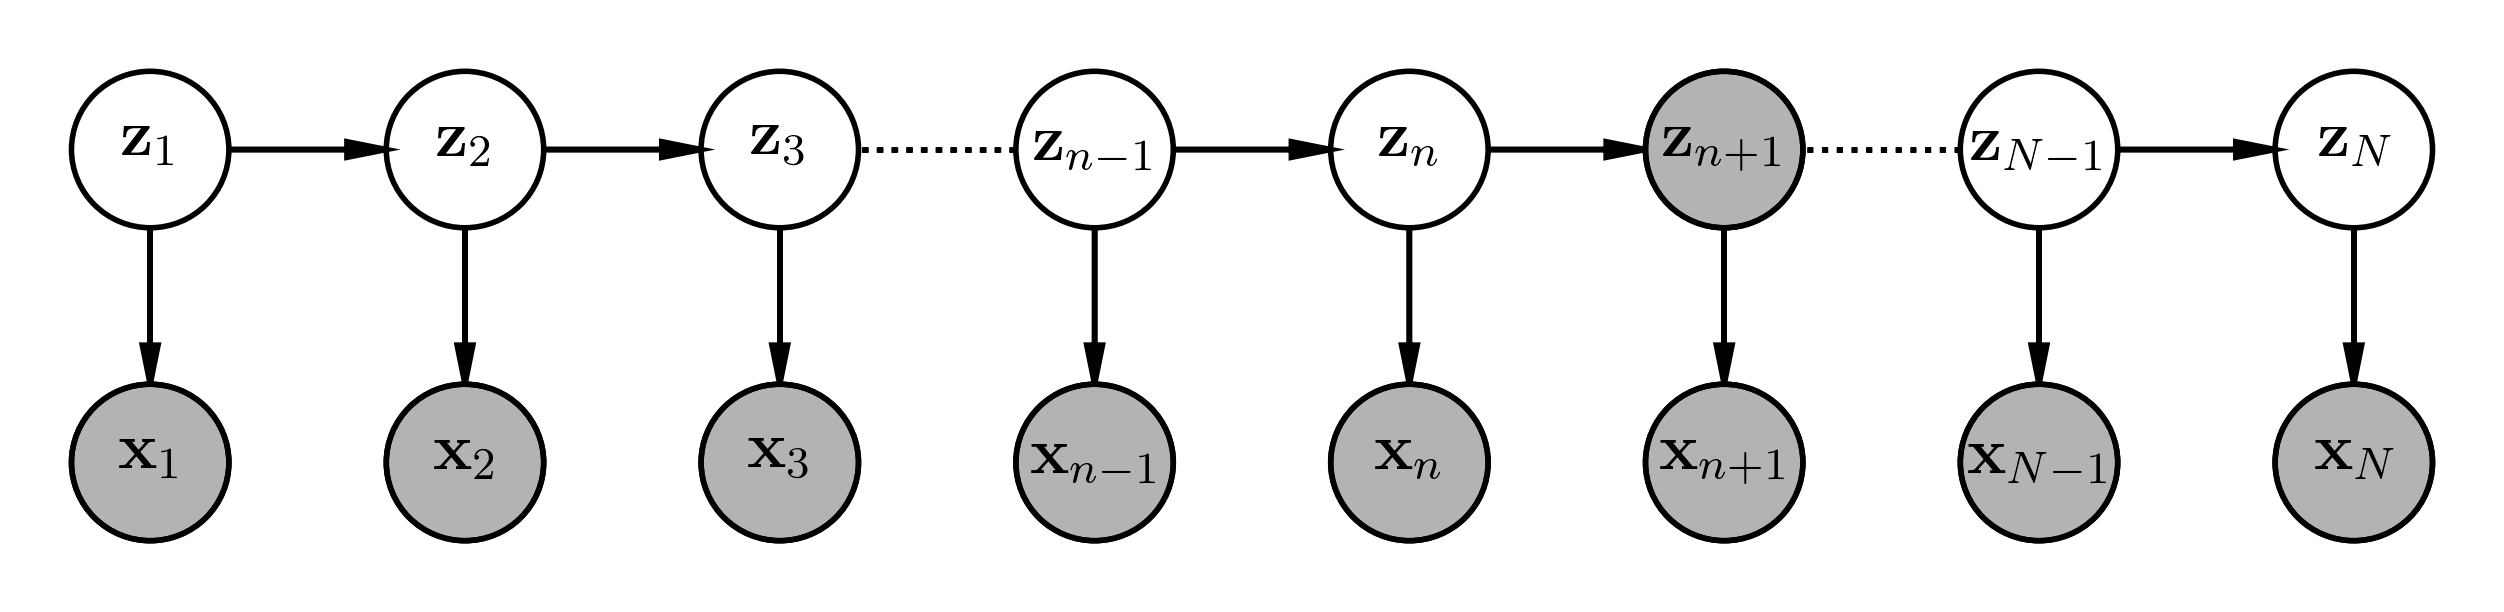
\includegraphics[width=10cm]{chain_n_plus_1_block.png}
\caption{$\bm{z}_{n+1}$ blocking $\bm{x}_{n+1}, \cdots, \bm{x}_N$ from $\bm{x}_n$}
\label{fig:chain_n_plus_1_block}
\end{figure}

By definition,
\begin{equation}
\begin{aligned}
p(\bm{z}_{n+1}|\bm{z}_n) &= \mathcal{N}(\bm{z}_{n+1}|A\bm{z}_n, \Gamma)\\
p(\bm{z}_{n}  | \bm{x}_1, \bm{x}_1, \cdots, \bm{x}_N)
&= \mathcal{N}(\bm{z}_{n+1}|\bm{\mu}_n, V_n)\\
\end{aligned}
\end{equation}
Then using identity \ref{eq:normal_reverse_conditional},
\begin{equation}
\begin{aligned}
p(\bm{z}_{n}|\bm{z}_{n+1}, \bm{x}_1, \bm{x}_1, \cdots, \bm{x}_N) =&
p(\bm{z}_{n}|\bm{z}_{n+1}, \bm{x}_1, \bm{x}_1, \cdots, \bm{x}_n)\\
=& \mathcal{N} ( \bm{z}_{n} | \bm{\mu}'_n, V'_n ) \\
\end{aligned}
\end{equation}
where
\begin{equation}
\begin{aligned}
V'_n &= \left(V_n^{-1} + A^T\Gamma^{-1}A\right)^{-1}\\
     &= V_n - V_n A^T\left(\Gamma + AV_nA^T\right)^{-1}AV_n\\
     &= V_n - K'_n AV_n\\
     &= (I - K'_n A)V_n\\
\end{aligned}
\end{equation}
and
\begin{equation}
\begin{aligned}
K'_n &=  V_n A^T\left(\Gamma + AV_nA^T\right)^{-1}\\
     &=  (V_n^{-1} + A\Gamma^{-1}A)^{-1}A^T\Gamma^{-1}\:\:\:\text{from identity}
\label{eq:define_K'_n}\ref{eq:matrix_inverse1}\\
\end{aligned}
\end{equation}
and
\begin{equation}
\begin{aligned}
\bm{\mu}'_n &= V'_n \left(A^T\Gamma^{-1}\bm{z}_{n+1} + V^{-1}_n\bm{\mu}_n\right)\\
&= (V^{-1}_n + A^T\Gamma^{-1}A)^{-1}A^T\Gamma^{-1}\bm{z}_{n+1} + (I - K'_n A)V_nV_n^{-1}\bm{\mu}_n\\
&= K'_n\bm{z}_{n+1} + (I - K'_n A)\bm{\mu}_n\:\:\text{ from equation\ref{eq:define_K'_n}}\\
\end{aligned}
\end{equation}

Now we are ready to derive
$p(\bm{z}_n, \bm{z}_{n+1} | \bm{x}_1, \bm{x}_1, \cdots, \bm{x}_N)$ and
$p(\bm{z}_n | \bm{x}_1, \bm{x}_1, \cdots, \bm{x}_N)$.
Let
$p(\bm{z}_n | \bm{x}_1, \bm{x}_1, \cdots, \bm{x}_N) = \mathcal{N}(\bm{z}_n | \bm{\mu}_{n}^{\gamma}, V_n^{\gamma})$.
From the equation \ref{dq:gaussian_joint},
\begin{equation}
\begin{aligned}
p(\bm{z}_{n+1}, \bm{z}_n | \bm{x}_1, \cdots, \bm{x}_N)
&= 
p(\bm{z}_{n} |\bm{z}_{n+1} ,\bm{x}_1, \bm{x}_2, \cdots, \bm{x}_N)
p(\bm{z}_{n+1} |\bm{x}_1, \bm{x}_2, \cdots, \bm{x}_N)\\
&= 
\mathcal{N}(\bm{z}_n|K'_n\bm{z}_{n+1} + (I - K'_nA)\bm{\mu}_n, V'_n)
\mathcal{N}(\bm{z}_{n+1} | \bm{\mu}_{n+1}^{\gamma}, V_{n+1}^{\gamma})\\
&= \mathcal{N}\Big(
\begin{bmatrix}
\bm{z}_{n+1}\\
\bm{z}_{n}\\
\end{bmatrix}
\Big|
\begin{bmatrix}
\bm{\mu}^{\gamma}_{n+1}\\
K'_n\bm{\mu}^{\gamma}_{n+1} + (I - K'_nA)\bm{\mu}_n\\
\end{bmatrix}
,
\begin{bmatrix}
V^{\gamma}_{n+1} & V^{\gamma}_{n+1}{K'_n}^T\\
K'_nV^{\gamma}_{n+1} & V'_n + K'_nV^{\gamma}_{n+1}K'_n\\
\end{bmatrix}
\Big)
\end{aligned}
\end{equation}
and
\begin{equation}
\begin{aligned}
p(\bm{z}_n | \bm{x}_1, \cdots, \bm{x}_N) &= 
\mathcal{N}\left(\bm{z}_n | 
K'_n\bm{\mu}^{\gamma}_{n+1} + (I - K'_nA)\bm{\mu}_n,\:
V'_n + K'_nV^{\gamma}_{n+1}K'_n
\right)\\
&=
\mathcal{N}\left(\bm{z}_n | \bm{\mu}^{\gamma}_{n}, V^{\gamma}_{n}\right)
\end{aligned}
\end{equation}
with the initial condition
\begin{equation}
\begin{aligned}
p(\bm{z}_N | \bm{x}_1, \cdots, \bm{x}_N)
&= 
\mathcal{N}\left(\bm{z}_N | \bm{\mu}^{\gamma}_{N}, V^{\gamma}_{N}\right)\\
&=
\mathcal{N}\left(\bm{z}_N | \bm{\mu}_{N}, V_{N}\right)
\end{aligned}
\end{equation}

For the EM algorithm, we need 
 $\mathbb{E}[\bm{z}_n]$, 
 $\mathbb{E}[\bm{z}_n\bm{z}_{n-1}^T]$, and
 $\mathbb{E}[\bm{z}_n\bm{z}_{n}^T]$ for the given $\bm{\mu}_0$, $P_0$, $A$, $\Gamma$, $C$, and $\Sigma$.
for the E-step.
They are given by
\begin{equation}
\begin{aligned}
\mathbb{E}[\bm{z}_n] &= \bm{\mu}^{\gamma}_n\\
\mathbb{E}[\bm{z}_n\bm{z}_{n}^T]  &= V^{\gamma}_{n} + \bm{\mu}^{\gamma}_n{\bm{\mu}^{\gamma}}^T_n\\
\mathbb{E}[\bm{z}_n\bm{z}_{n-1}^T] &=
 V^{\gamma}_{n}{K'}_{n-1}^T + \bm{\mu}^{\gamma}_n{\bm{\mu}^{\gamma}}^T_{n-1}
\end{aligned}
\end{equation}
For the M-step, which maximizes $\bm{\mu}_0$, $P_0$, $A$, $\Gamma$, $C$, and $\Sigma$, please see pp 642, 643, 13.3.2 of PRML \cite{bishop2007}.


\bibliography{baum_welch_viterbi_kalman.bib}{}
\bibliographystyle{plain}


\end{document}
